\section{Softwarearchitektur (8P)}

\subsection{Gewählte Architektur (4P)}
\task{In der Vorlesung wurden Softwarearchitekturen vorgestellt. Welche Architektur wurde davon umgesetzt? Analyse und Begründung inkl. UML der wichtigsten Klassen, sowie Einordnung dieser Klassen in die gewählte Architektur}

\subsubsection*{Analyse}
Unser Projekt Bilanzius basiert auf einem klassischen 3-Schichtenmodell. Ziel dieser Architektur ist es, die Verantwortlichkeiten klar zu trennen und eine lose Kopplung zwischen den Komponenten zu ermöglichen. Die drei Hauptschichten sind:
\begin{enumerate}
    \item \textbf{Präsentationsschicht} \newline 
    Diese Schicht stellt die Schnittstelle zur Benutzerinteraktion dar. In unserem Fall besteht sie hauptsächlich aus der \texttt{Main}-Klasse, die Benutzereingaben verarbeitet und an die entsprechenden Komponenten weiterleitet.
    \item \textbf{Domänenschicht (Domain Layer)} \newline
    Die zentrale Schicht enthält die gesamte Geschäftslogik. Hier befinden sich:
    \begin{itemize}
        \item 
        Die \textbf{Command-Klassen}: Jede Klasse repräsentiert einen ausführbaren Befehl (z.B. \texttt{/help}, \texttt{/exit}).
        \item 
        Der \textbf{CommandController}: Dieser dient als Vermittler und Dispatcher zwischen Eingaben der Präsentationsschicht und ausführbaren Commands.
        \item 
        Die \textbf{Service-Interfaces} wie BankAccountService, UserService usw., die fachliche Operationen definieren.
    \end{itemize}
    \item \textbf{Datenschicht (Data Layer)} \newline
    Diese Schicht kapselt den Zugriff auf die persistente Datenhaltung (SQLite). Die konkreten Implementierungen der Service-Interfaces (\texttt{SqliteBankAccountService}, \texttt{SqliteUserDatabaseService}, usw.) befinden sich hier. Sie sind über das Repository \texttt{DatabaseServiceRepository} zentral angebunden.
\end{enumerate}

\subsubsection*{Begründung}
Wir haben uns für dieses Schichtenmodell entschieden, weil es:
\begin{itemize}
    \item eine klare Strukturierung bei wachsender Komplexität bietet
    \item dadurch einfach erweiterbar ist
    \item eine lose Kopplung zwischen den Komponenten bietet
    \item gut mit den Prinzipien von Domain Driven Design kombinierbar ist
\end{itemize}

\subsubsection*{UML-Diagramm}
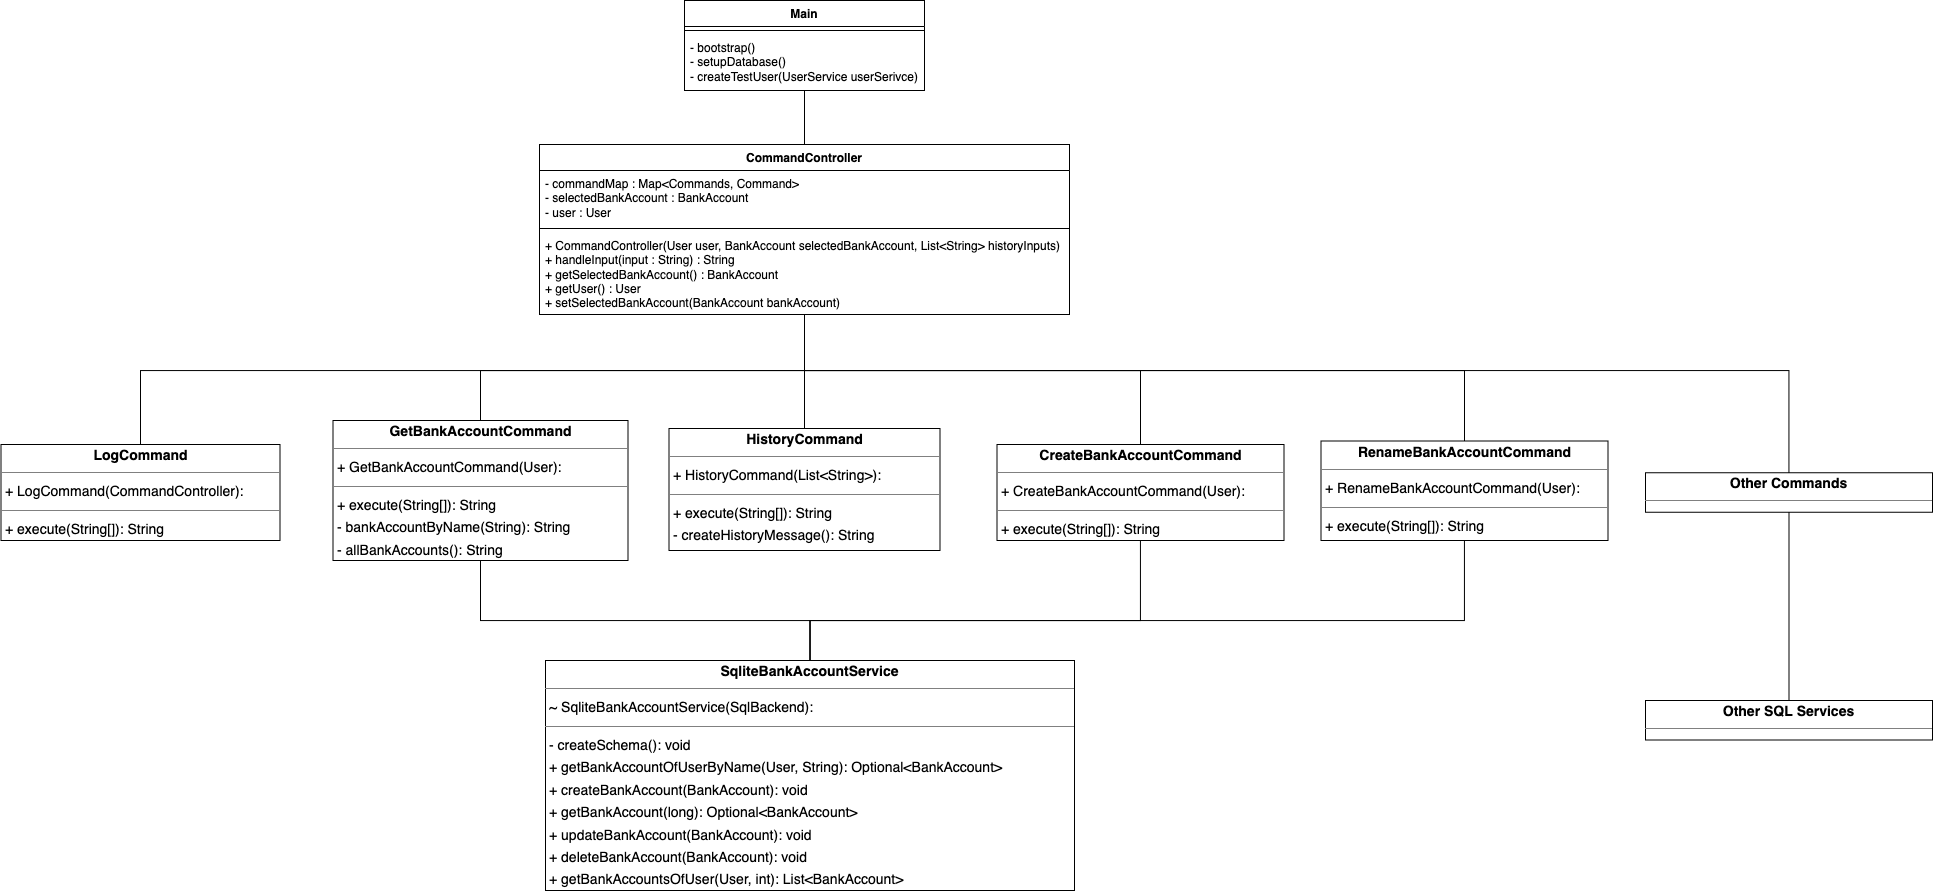
\includegraphics[width=\linewidth]{kapitel2_architektur/Softwarearchitekturen.drawio.png}



\subsection{Domain Code (1P)}
\task{kurze Erläuterung in eigenen Worten, was Domain Code ist – 1 Beispiel im Code zeigen, das bisher noch nicht gezeigt wurde}
Domain Code ist der Teil einer Anwendung, der die eigentliche \textbf{Geschäftslogik} beschreibt – also die Regeln, Abläufe und Begriffe der realen Welt, die mit der Software abgebildet werden sollen. Im Gegensatz zu technischem Code (z.B. Datenbank, UI) steht hier die fachliche Bedeutung im Vordergrund. Der Domain Code ist direkt von der Problemdomäne inspiriert und sollte möglichst klar und unabhängig von der Infrastruktur sein.

\subsubsection*{org.bilanzius.persistence.models.Transaction}
\lstinputlisting[language=Java,style=codeStyle]{kapitel2_architektur/ddd1.java}



\subsection{Analyse der Dependency Rule (3P)}
\task{In der Vorlesung wurde im Rahmen der ‘Clean Architecture’ die s.g. Dependency Rule vorgestellt. Je 1 Klasse zeigen, die die Dependency Rule einhält und 1 Klasse, die die Dependency Rule verletzt;   jeweils UML (mind. die betreffende Klasse inkl. der Klassen, die von ihr abhängen bzw. von der sie abhängt) und Analyse der Abhängigkeiten in beide Richtungen (d.h., von wem hängt die Klasse ab und wer hängt von der Klasse ab) in Bezug auf die Dependency Rule}

\subsubsection*{Positiv-Beispiel: Dependency Rule}
Der \texttt{CommandController} verarbeitet Nutzereingaben und delegiert die Ausführung an sogenannte Commands. Dabei kennt er nur das \textbf{Interface} \texttt{Command} – und nicht die konkreten Implementierungen. Das bedeutet:
\begin{itemize}
    \item Die Abhängigkeit zeigt nach innen, also zur Domänenschicht.
    \item Der Controller bleibt unabhängig von technischen Details.
    \item Konkrete Commands können sich ändern oder erweitert werden, ohne dass der CommandController geändert werden muss.
\end{itemize}

\begin{figure}[htbp]
    \centering
    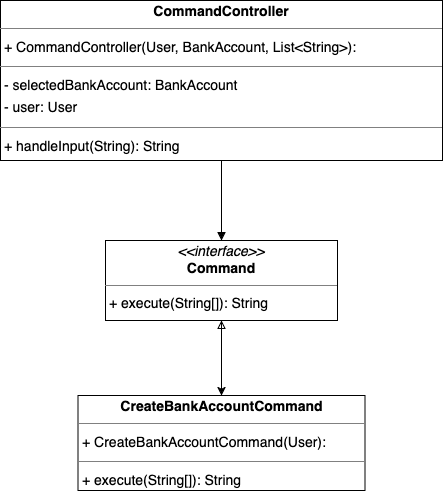
\includegraphics[width=0.7\linewidth]{kapitel2_architektur/DepRulPos.png}
\end{figure}


Hinweis: Weitere Commands wie \texttt{HelpCommand}, \texttt{ExitCommand} usw. implementieren ebenfalls das Interface \texttt{Command}, sind aber aus Platzgründen nicht dargestellt.

\subsubsection*{Negativ-Beispiel: Dependency Rule}
Die \texttt{SignUp}-Klasse ist verantwortlich für die Registrierung bzw. Anmeldung von Nutzern. Allerdings vermischt sie mehrere Ebenen der Anwendung in einer einzigen Klasse:
\begin{itemize}
    \item Sie greift auf \textbf{Datenbankservices} zu (\texttt{DatabaseProvider}, \texttt{UserService}).
    \item Sie interagiert mit dem \textbf{CLI-Interface} (\texttt{IOContext}).
    \item Sie verwendet \textbf{Utility-Logik} (\texttt{Localization}).
\end{itemize}
Dadurch verletzt \texttt{SignUp} die Dependency Rule gleich mehrfach:
\begin{itemize}
    \item Die Klasse kennt sowohl \textbf{Domänen- als auch Infrastrukturelemente}.
    \item \textbf{Abhängigkeiten verlaufen in beide Richtungen}, was die Wartbarkeit und Testbarkeit erschwert.
\end{itemize}

Hier hängt die fachlich zentrale Klasse direkt von mehreren äußeren Schichten ab – Verletzung der Clean Architecture Grundsätze.

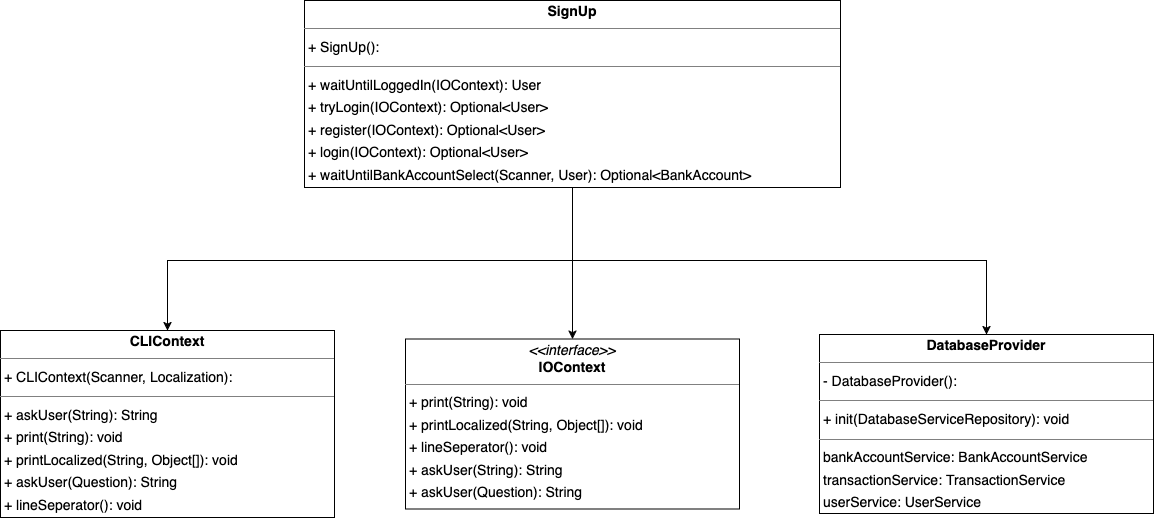
\includegraphics[width=\linewidth]{kapitel2_architektur/DepRulNeg.png}